%%%
%%% Annual Cognitive Science Conference
%%% Sample LaTeX Paper -- Proceedings Format
%%%

% Original : Ashwin Ram (ashwin@cc.gatech.edu)       04/01/1994
% Modified : Johanna Moore (jmoore@cs.pitt.edu)      03/17/1995
% Modified : David Noelle (noelle@ucsd.edu)          03/15/1996
% Modified : Pat Langley (langley@cs.stanford.edu)   01/26/1997
% Latex2e corrections by Ramin Charles Nakisa        01/28/1997
% Modified : Tina Eliassi-Rad (eliassi@cs.wisc.edu)  01/31/1998
% Modified : Trisha Yannuzzi (trisha@ircs.upenn.edu) 12/28/1999
% Modified : Mary Ellen Foster (M.E.Foster@ed.ac.uk) 12/11/2000
% Modified : Ken Forbus                              01/23/2004
% Modified : Eli M. Silk (esilk@pitt.edu)            05/24/2005
% Modified : Niels Taatgen (taatgen@cmu.edu)         10/24/2006
% Modified : David Noelle (dnoelle@ucmerced.edu)     11/19/2014
% Modified : Roger Levy (rplevy@mit.edu)             12/31/2018
% Modified : Stephanie Denison                       11/29/2025
% Modified : Dae Houlihan (daeda@mit.edu)            12/01/2025


%%% Change "letterpaper" in the following line to "a4paper" if you must.

\documentclass[10pt,letterpaper]{article}

\usepackage{cogsci}

% \cogscifinalcopy %%% Uncomment this line for the final submission

%%% Bibliography %%%
\usepackage[
  style=apa,
  natbib=true,
  annotation=false,
]{biblatex}
\addbibresource{../references.bib} %%% Specify the path to a BibLaTeX file
\setlength{\bibhang}{.125in}

\usepackage{float} %%% Roger Levy added this and changed figure/table placement to [H] for conformity to Word template, though floating tables and figures to top is still generally recommended!

%%% Additional packages from original manuscript
\usepackage{amsmath}
\usepackage{graphicx}
\usepackage{booktabs}
\usepackage{multirow}
\usepackage{url}
\urlstyle{same}

% Sometimes it can be useful to turn off hyphenation for purposes such as spell checking of the resulting PDF.
% \usepackage[none]{hyphenat} %%% Uncomment to turn off hyphenation

\title{Inference of Numerical Competence from Speed and Accuracy}

%%% Format authors using helper functions from authblk package %%%
\author[1]{Anonymous CogSci submission}
\affil[1]{}

%%% Or, format authors manually %%%
% \author{
%   {\large\bfseries Author N. One (a1@uni.edu)$^1$ \& Author Number Two$^2$} \\
%   {\normalsize\normalfont
%     $^1$Department of Hypothetical Sciences, University of Illustrations \\
%     $^2$Department of Example Studies, University of Demonstrations
%   }
% }

\begin{document}

\maketitle

\begin{abstract}
People routinely infer others' competence under uncertainty, often relying on cues such as task's difficulty and past accuracy. An emerging body of research suggests that people approximate Bayesian inference when doing so. We extend these results by testing whether people can infer other's numerical ability in a way consistent with a rational Bayesian model. In Study 1, we found that participants accurately predicted math performance of another individual from information about past accuracy. Computational modelling shows that participants' inferences are better described by Bayesian processes than by plausible heuristics. Study 2 introduce a modified paradigm, where participants are told about both the past accuracy and speed of solving a problem. We found that, although participant are quite accurate in their predictions, they do not seem to take into account information about speed.

\textbf{Keywords:}
Computational Modeling;
 Social Cognition;
  Competence;
 Knowledge Attribution;
 Information Search
\end{abstract}

% \section{Introduction}\label{introduction}

% Humans often make consequential decisions that hinge on judgments of others’ competence: whom to ask for advice, who should lead, or be hired (e.g., \citealt{Garfield-2025,Harris-2018,Cuddy-2011}). However, assessing someone's else competence might requires sophisticated inferences \citep{Jones-1989}. Imagine that you have to choose between two teachers, with limited information about them. If you observe one of them solving an easy task and the other one failing a hard task you might have trouble to choose as it does not change your prior expectations about their competence.

% People routinely infer others' competence from such limited information \citep{Dubourg-2025,Mercier-2025c,Jara-Ettinger-2015a}. As many aspect of our social cognition, competence evaluation can be viewed as a probabilistic inference under uncertainty. An emerging body of evidence show that people approximate Bayesian inference when doing so \citep{Baker-2017,Davis-2025,Jara-Ettinger-2017,Xiang-2026}. More specificaly, \citet{Mercier-2025c} have shown that participant can infer the pieces of knowledge that someone possess when given access to information about a success or failure in answering a general knowledge question. Using a naturalistic paradigm with trivia questions, they show that participants can leverage their prior about the average ability of the population in a domain (e.g American History) and optimally integrate new information to update their estimation of competence.

% Nevertheless, \citep{Mercier-2025c} only tested their model in a facet of competence (knowldgeability) while claiming that their model is generalist. We may also wish to infer whom to trust, learn from, or collaborate with based on their skills. The present study investigates whether the findings of \citep{Mercier-2025c} generalize to skill-based competence, numerical competence in particular, using arithmetic problems as materials. While the trivia-based studies tested inferences about knowledge, here we examine whether individuals can judge another’s skill level from sparse information about prior performance.

% \subsection{Computational Model}\label{computational-model}

% Inferring competence, even from past accuracy and difficulty, is far from straightforward \citep[e.g.,][]{Jones-1989}. To account for stochastic outcomes (e.g., guessing or slipping), rational observers must integrate new evidence with prior expectations. We formalize this using the Bayesian framework validated in previous literature \citep{Mercier-2025c, Jansen-2021}.

% This framework posits that observers hold a generative model linking latent competence to performance via a psychometric function (based on Item Response Theory). When an observer sees an individual succeed (\(S=1\)) or fail (\(S=0\)) at a task of known difficulty \(\beta\), they update their prior beliefs about that individual's competence \(\theta\) according to Bayes' rule. 

% \begin{equation}
% p(\theta \mid \beta, S) \propto p(S \mid \beta, \theta) \cdot p(\theta)
% \label{eq:bayes}
% \end{equation}

% This process allows for optimal predictions of future performance by integrating the likelihood of the observed outcome with the prior distribution of competence in the population. The specific mathematical formalization, including the likelihood functions and parameter definitions, is detailed in the Methods section of Study 1.

\section{Introduction}\label{introduction}

Humans routinely make decisions that depend on judgments of others’ competence: whom to ask for advice, whom to hire, or whom to cooperate with \citep{Harris-2018,Cuddy-2011,Xiang-2023}. Yet competence is not directly observable. Observers must infer it from sparse and noisy cues, and even apparently informative outcomes can be ambiguous \citep{Jones-1989}. Consider choosing between two teachers after observing a single performance each: one solves an easy problem, the other fails a hard one. Despite the contrast between success and failure, neither observation is very diagnostic, because easy successes and hard failures are both common.

A growing body of work suggests that people nonetheless make competence inferences that approximate rational probabilistic reasoning \citep{Baker-2017,Davis-2025,Jara-Ettinger-2017,Xiang-2026,Jansen-2021,Aboody-2025}. In particular, \citet{Mercier-2025c} used a naturalistic trivia paradigm to show that participants infer what others know from minimal evidence (a single success or failure), by combining the observed outcome with prior expectations about item difficulty and the average competence of the population in a domain. In this framework, competence judgments integrate (i) the diagnosticity of the observed performance—success on a hard item is more informative than success on an easy one—and (ii) prior beliefs about how competence varies across individuals.

However, previous research primarily concern knowledgeability, a facet of competence \citep{Aboody-2025,Dubourg-2025,Mercier-2025c}. This leaves open a key question about generality: do people apply similar inference principles to skill-based competence? Many everyday judgments involve problem solving rather than the static retrieval of stored facts (e.g., mental arithmetic, programming). Here we test whether the same inferential logic extends to numerical competence, using arithmetic problems that vary in difficulty under a strict time limit.

Our contribution is twofold. First, in Study~1 we adapt the trivia paradigm of \citet{Mercier-2025c} and \citet{Dubourg-2025} to arithmetic and test whether participants’ judgments about another person’s numerical ability are consistent with a Bayesian model that links latent competence to success probabilities across item difficulties. We also compare this normative account to heuristic baselines previously considered in the trivia domain \citep{Mercier-2025c}. 

Second, in Study~2 we test whether observers additionally use speed as a cue to competence when accuracy information is held constant. While speed is often cited as a marker of arithmetic fluency \citep{Roy-2025,Cheng-2021}, it is theoretically ambiguous: faster responses may signal efficiency, but they can also reflect lower response caution, whereas for complex reasoning tasks, competent individuals often take longer to verify their answers \citep{Goldhammer-2011,Hedge-2018,Richardson-2022,Berke-2023}. We therefore ask whether people’s competence judgments track the true diagnostic value of response time in our task.

\subsection{Computational Model}\label{computational-model}

Inferring competence from performance requires accounting for uncertainty: people can guess, slip, or make occasional errors even when skilled \citep{Jones-1989}. We formalize competence inference using the Bayesian framework developed in \citet{Mercier-2025c} and closely related to item-level models of ability \citep{Jansen-2021}. Observers are assumed to represent a latent competence parameter $\theta$ for an individual and a known item difficulty parameter $\beta$ for each task. After observing whether an individual succeeds ($S=1$) or fails ($S=0$) on an item of difficulty $\beta$, observers update beliefs about $\theta$ via Bayes’ rule:
\begin{equation}
p(\theta \mid \beta, S) \propto p(S \mid \beta, \theta)\, p(\theta).
\label{eq:bayes}
\end{equation}

The likelihood $p(S \mid \beta, \theta)$ links competence and difficulty through a psychometric function (an IRT-style mapping), allowing outcomes to be stochastic rather than deterministic. Given the posterior over $\theta$, the observer can then predict performance on new items by marginalizing over uncertainty in competence. The full specification of the likelihood and the prediction rule, along with model comparisons against heuristic baselines, is provided in the Methods for Study~1.

\section{Study 1}\label{study-1}

In this study, we use a paradigm similar to \citet{Mercier-2025c} to investigate the inferences people make about individuals who provide either a correct or incorrect answer to a math question. We predicted that participants' behavior be best captured by the optimal Bayesian Model. More precisely, we put forward the following hypotheses\footnote{The procedures, data collection, analysis plan and the models were pre-registered for Study 1 and 2: \url{https://osf.io/aecyr/?view_only=2b8fc0d1c99e450f8b8534e2aab83a92}. Data and code are openly availble: \url{https://osf.io/aecyr/files/github?view_only=2b8fc0d1c99e450f8b8534e2aab83a92 }}:

\textbf{H1.} For different questions, participants can accurately assess the rarity of reaching an accurate answer within the time-limit.

\textbf{H2.} On average, participants' predictions of the probabilities of success on different questions, given the observation of a failure/success on a particular question, will be significantly correlated with true conditional probabilities.

\textbf{H3.} The predictions of the Main Model are positively correlated with participants' average predictions.

\textbf{H4.} When fitted to the aggregated dataset, the Main Model better captures participants' behavior than heuristic models.

\subsection{Methods}\label{methods}

\subsubsection{Participants}\label{participants-1}

300 U.S. participants were recruited via Prolific. We applied pre-registered exclusions for inattentiveness/LLM use (N = 2), suspected use of external calculation aids (N = 35), and manipulation noncompliance (changing the pre-ticked success/failure response; N = 39), leaving a sample of 224 (120 women, 104 men, \(M_{Age}\) = 43.4, \(SD_{Age}\) = 14.8)

\subsubsection{Procedure}\label{behavioral-task}

This experiment replicate the paradigm of \citet{Mercier-2025c}, but with different stimuli and a time constraint. Participants were asked to complete two phases. In the judgement phase, they were asked to evaluate five virtual agents on a set of fifteen mathematical questions. Participants were told that in order to help them, they will have access to the performance of the virtual agent on one of the questions. For each trial, participants were assigned to a Success/Failure condition: each virtual agent correctly ("Success" condition) or incorrectly ("Failure" condition) answered the question under 30 seconds. The specific question shown was randomly drawn from the stock of 15 questions. Only the question, and whether the virtual agent got it right or not, was provided to the participants, but not the specific answer. We call this item the "observed question."

Participants were then asked to evaluate whether the virtual agent succeeded or failed to answer the other 14 questions from the quiz within the time limit. We call each of these items a "new question." Observed-new questions pairs are thus, for each observed questions, the 14 predictions on new questions. They also had to estimate how many people, out of 100, correctly answered the observed question within 30 seconds.

In the second phase, participants had to complete the 15 maths questions, and one additional question designed to detect those using external tools. Questions' order was randomly determined. They were instructed that they had to answer each question under 30 seconds. At any time, once they had entered an answer, they could click Submit to proceed. At 15 seconds and 25 seconds time warnings appeared. If after 30 seconds they had not submitted an answer, the survey automatically proceeded to the next question and the timer restarted.

\subsubsection{Materials}\label{materials}

The arithmetic stimuli were designed to establish a difficulty gradient following principles by Dehaene (2011). We manipulated five parameters to vary complexity: (1) answer magnitude (number of digits); (2) semantic roundness (operands ending in zeros vs. "sharp" non-zero integers); (3) operand count; (4) carry-over frequency (aggregate sums >10); and (5) placeholder tracking (alignment required for variable-length operands). For example, the problem 100,034,090 + 1,023 represents a high-difficulty item as it requires placeholder tracking, mixed sharp/round operands, and a carry-over operation.

\subsubsection{Computational Models}\label{computational-models}
We used the Bayesian/IRT framework from \citet{Mercier-2025c}. Each question is assigned a difficulty score \(\beta\) by averaging judged difficulty ratings (divided by 100) and applying a logit transform to map scores from (0,1) to an unbounded scale.\footnote{This transformation is inspired by the way difficulty is operationalized in frameworks like Item Response \citet{Rasch-1960}. The qlogis transform is given by: \(qlogis(p) = log(p/(1-p))\).} Competence \(\theta\) has a normal prior \(\theta \sim \mathcal{N}(\mu,\sigma^2)\), and success is stochastic under a normal-ogive Rasch likelihood:
\begin{equation}
p(S=1 \mid \beta,\theta)=\Phi\!\left(\frac{\theta-\beta}{\varepsilon}\right)
\end{equation}
After observing \((\beta_{\text{obs}}, S_{\text{obs}})\), the posterior is proportional to \(p(S_{\text{obs}}\mid \beta_{\text{obs}},\theta)\,p(\theta)\). The predicted success on a new item is
\begin{multline}
P(S=1 \mid \beta_{\text{new}},\beta_{\text{obs}},S_{\text{obs}})= \\
\int \Phi\!\left(\frac{\theta-\beta_{\text{new}}}{\varepsilon}\right)
p(\theta \mid \beta_{\text{obs}},S_{\text{obs}})\,d\theta.
\end{multline}
The Bayesian model has four free parameters: \(\mu,\sigma^2,\varepsilon\), and a softmax temperature \(\tau\) that maps probability estimates to binary responses. We compare this model to the same two heuristic baselines (Threshold, Anchor) described in \citet{Mercier-2025c}.

The Threshold heuristic assumes a deterministic rule: after a success, competence is at least the observed difficulty; after a failure, competence is at most that difficulty. It treats all values as equally likely, then predicts success on a new item by the posterior mass above its difficulty (with \(\tau\) governing response noise). The Anchor heuristic collapses inference to a single point estimate: after success, competence is set a fixed distance \(\Delta\) above the observed difficulty; after failure, \(\Delta\) below. It then predicts success deterministically for items easier than that anchor (again with \(\tau\) for response noise).

\subsection{Results}

\paragraph{Difficulty judgments (H1).}
Participants’ perceived difficulty of each item closely tracked objective difficulty (i.e. the percentage of participants not being able to solve an item within the time limit in the questionnaire phase). A linear mixed-effects model predicting objective difficulty from perceived difficulty yielded a strong positive association ($\beta = 0.45$, $t(911.69)=22.18$, $p<.001$; see Figure~\ref{fig:S1-fig-behav}A).

\paragraph{Competence inferences from a single outcome (H2).}
Participants used the observed success/failure to make graded predictions about performance on other items. Averaged conditional predictions were strongly correlated with the true conditional probabilities computed from participants’ own test performance ($\beta = 0.86$, $t(418)=34.72$, $p<.001$, $R^2_{\text{adj}}=0.74$; Figure~\ref{fig:S1-fig-behav}B).

\paragraph{Model comparison (H3--H4).}
The Bayesian/IRT model reproduced participants’ average conditional predictions across item pairs (Main Model: $\beta = 0.94$, $t(418)=58.29$, $p<.001$, $R^2_{\text{adj}}=0.89$), outperforming both heuristic baselines (Threshold: $R^2_{\text{adj}}=0.39$; Anchor: $R^2_{\text{adj}}=0.59$; Figure~\ref{fig:S1-fig-model-comparison}). Model selection using BIC favored the Bayesian model over Threshold and Anchor ($BIC_{\text{Bayes}}=16063.72$, $BIC_{\text{Threshold}}=19411.92$, $BIC_{\text{Anchor}}=18259.96$), providing strong evidence for the Bayesian account.

\paragraph{Inferences among low-performing participants (H1m--H2m).}
To test whether accurate competence inference requires high arithmetic ability, we repeated H1--H2 in the bottom 30\% of performers on the arithmetic test. Even in this subsample, perceived difficulty tracked objective difficulty (H1m: $\beta = 0.93$, $t(303)=44.51$, $p<.001$), and average conditional predictions remained strongly correlated with true conditional probabilities (H2m: $\beta = 0.85$, $t(448)=34.03$, $p<.001$, $R^2_{\text{adj}}=0.72$).


% Estimating others' competence relies on the participants assuming that performance on the arithmetic questions is nested, with people successfuly answering hard questions being also able to answer easier ones, but not vice-versa. In order to make use of the nestnessness of the questions, participants additionally needed to accurately assess the difficulty of reaching a correct answer in the time limit for different questions.

% The arithmetic questions were manipulated to be nested by varying their difficulty. To verify that this manipulation resulted in nestedness of participant performance, two nestedness measures, NODF and Temperature, were calculated from a binary matrix of participants' successes/failures on each question. Each metric was computed using the oecosimu() function in the vegan package in R (Oksanen et al.~2013). The observed nestedness values (NODF or Temperature) were compared to a simulated distribution of possible values under the null hypothesis that the arithmetic questions were not nested. A higher, positive NODF indicates greater nestedness, while a lower, negative Temperature indicates greater nestedness. The primary manipulation check (\textbf{MC1}) was confirmed for both measures, with a significantly higher NODF and lower Temperature than under the null model (NODF: Z = 20.29, p = .002; Temperature: Z = -12.67, p = .002). This confirmed that participants who succeeded on hard questions (rarely answered correctly) also tended to succeed on easier ones (more commonly answered correctly). A secondary manipulation check (\textbf{MC1'}), directly derived from nesting, was then performed to check that, on average, the more difficult the question the higher the average performance score of those who got it right. Fitting a linear model with average performance score as the predictor and objective question difficulty (the rarity of answering correctly within the time limit) as the outcome, the secondary manipulation check was supported as the estimate was significantly positive (\(\beta\) = 0.24, t(13) = 13, p = \textless{} .001, Adjusted \(R^2\) = 0.92).

% As a pre-requisite for the participants making use of the nested nature of the questions to infer which questions the virtual agent got right, they must be able to judge the difficulty of the questions. More specifically, they must be able to accurately assess the rarity of reaching an accurate answer within the time-limit for different questions. This was our first hypothesis (\textbf{H1}). We fit a linear mixed effects model predicting true question difficulty (the inverse of the true percentage of people who could answer correctly on the arithmetic test) with participants' perception of the question difficulty (the inverse of the percentage of people they predict could answer correctly) as the fixed effect, and random effects for participants. Confirming \textbf{H1}, the fixed effect estimate for perceived difficulty was significantly positive (\(\beta\) = 0.45, t(911.69) = 22.18, p = \textless{} .001). The high correlation between perceived difficulty and true difficultyis visible in Figure \ref{fig:S1-fig-behav}A.

\begin{figure}

{\centering 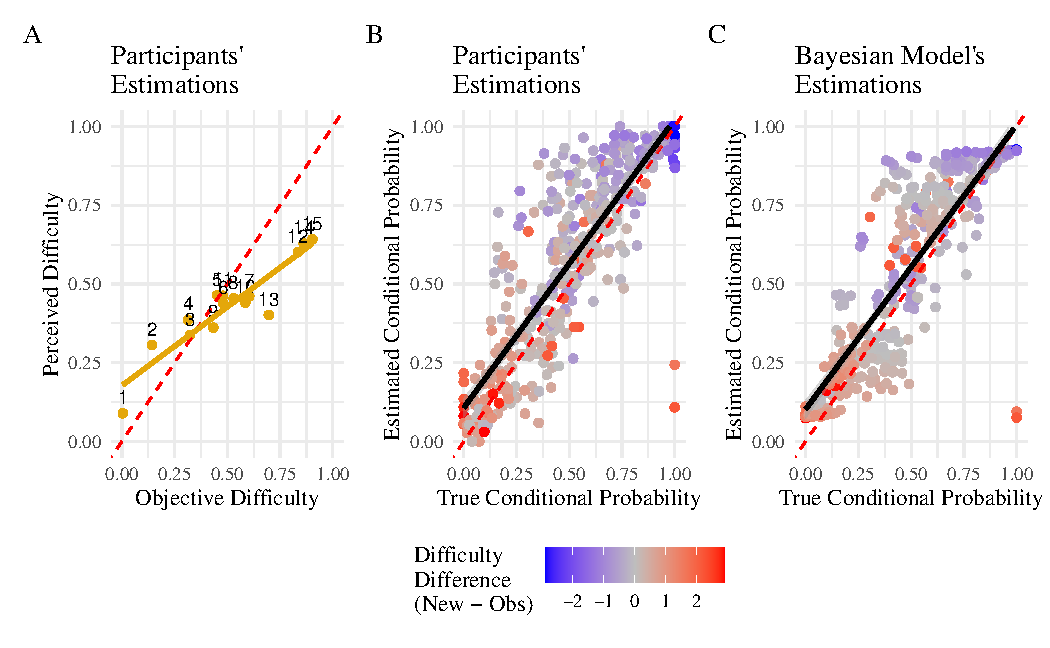
\includegraphics[width=0.9\linewidth]{../figures/S1-fig-behav-1}

}

\caption{(\textbf{A}) Each question's estimated difficulty as a function of its true difficulty. Numbers refer to the question ID (see Materials). The red dashed line represents a perfectly accurate estimation. (\textbf{B}) Participants' estimated probability of answering a new question correctly, conditioned on the performance on the observed question, as a function of true conditional probabilities. (\textbf{C}) Our Bayesian model's estimated conditional probabilities as a function of true conditional probabilities. For (\textbf{B}) and (\textbf{C}), each data point corresponds to the average values for a pair of two questions: one for which the individual's performance is observed, and one for which the individual's performance has to be guessed. The red line represents a perfectly accurate prediction, while the dark line represents the fit of the linear model.}\label{fig:S1-fig-behav}
\end{figure}

% Participants were able to use their accurate judgments of question difficulty to then infer the arithmetic competence of another based on the observation of their success or failure on just one specific question. We aggregated their judgments of which questions would be answered correctly, conditional on success or failure on the observed question. These are the estimated conditional probability values. Then, from the participants' answers to the arithmetic questions, we computed the True Conditional Probability of answering a new question given another question was successfully answered. Our second hypothesis (\textbf{H2}) was that, on average, participants' estimations of the probabilities of success for different questions, given the observation of success/failure on a particular question, would be significantly correlated with true conditional probabilities. A linear model with the average estimated conditional probability as an dependent variable and the true conditional probability as the independent variable and confirmed participants were able to predict the true conditional probability with a great precision (\(\beta\) = 0.86, t(418) = 34.72, p \textless{} .001, Adjusted \(R^2\) = 0.74). The strong correlation between average estimated conditional probability and true conditional probability is visualized in Figure \ref{fig:S1-fig-behav}B.

% We also found that participants did not have to be arithmetically competent themselves to make reasonable inferences about the competence of others. We tested whether the 30\% of participants who performed worst on the arithmetic test could still judge the difficulty of the questions (\textbf{H1m}) and whether they could accurately infer the conditional probability of answering a new question given an observed question and outcome (\textbf{H2m}). Confirming H1m with a linear mixed effect model, we found that the worst performers' perception of question difficulty was highly correlated with objective question difficulty, just as much as the for the full set of participants (\(\beta\) = 0.93, t(303) = 44.51, p \textless{} .001).

% Confirming H2m with a linear model, we found that the worst performers' were still very accurate in predicting which other questions the virtual agent would succeed at, with a high correlation between true and judged conditional probabilities (\(\beta\) = 0.85, t(448) = 34.03, p \textless{} .001, Adjusted \(R^2\) = 0.72).

% \subsection{Modelling Results - Confirmatory Analyses}\label{modelling-results---confirmatory-analyses}

% To interrogate the predictive power of our the Bayesian Model, we tested three main hypotheses: (\textbf{H3}) posited that the predictions of the Main Model would be positively correlated with participants' average predictions. In addition, we hypothesized that, when fitted to the aggregated dataset, the Main Model would better capture participants' behavior than the Threshold heuristic model (\textbf{H4}) and the Anchor heuristic model (\textbf{H5}).

% For each model, we determined the optimal free parameters by maximizing the log-likelihood of participants' responses, given the specific model and its parameter set.

% \[
% \mathcal{L}(\mathcal{M}_1 \mid x) = \sum_{i=1}^{N} y_i \log  P(p(x_i)) + (1 - y_i) \log (1- p(x_i))
% \]

% In the Main model, we varied the prior mean (\(\mu\)) between 0 and 1, the standard deviation (\(\sigma\)) between 0.05 and 1, the noise parameter between 0.05 and 1, and the beta parameter of the softmax function between 0 and 10. In the Threshold heuristic model, only the beta parameter was varied. In the Anchor heuristic model, both the beta parameter and the difficulty parameter were adjusted. All models received the following inputs: the fact that the virtual agent succeeded (\(S = 1\)) on a question with perceived difficulty \(D_{\text{obs}}\), and a request to predict the likelihood of success on a new question with perceived difficulty \(D_{\text{new}}\).

% Investigating \textbf{H3}, we fit three linear models to compare the Main Model's and the two heuristic models' fit with participants' answers, as well as how much variance in participant behaviour they explained. We found that our Main Model was very strongly correlated with participant behaviour (\(\beta\) = 0.94, t(418) = 58.29, p \textless{} .001, Adjusted \(R^2\) = 0.89). The Threshold model showed lower correlation with the data (\(\beta\) = 0.63, t(418) = 16.40, p \textless{} .001, Adjusted \(R^2\) = 0.39). The Anchor model was the weakest fit to the data (\(\beta\) = 0.77, t(418) = 24.39, p \textless{} .001, Adjusted \(R^2\) = 0.59). Figure \ref{fig:S1-fig-model-comparison} shows participants' average prediction for each possible pair of arithmetic questions (observed and judged) compared to the three models' predictions.

\begin{figure}

{\centering 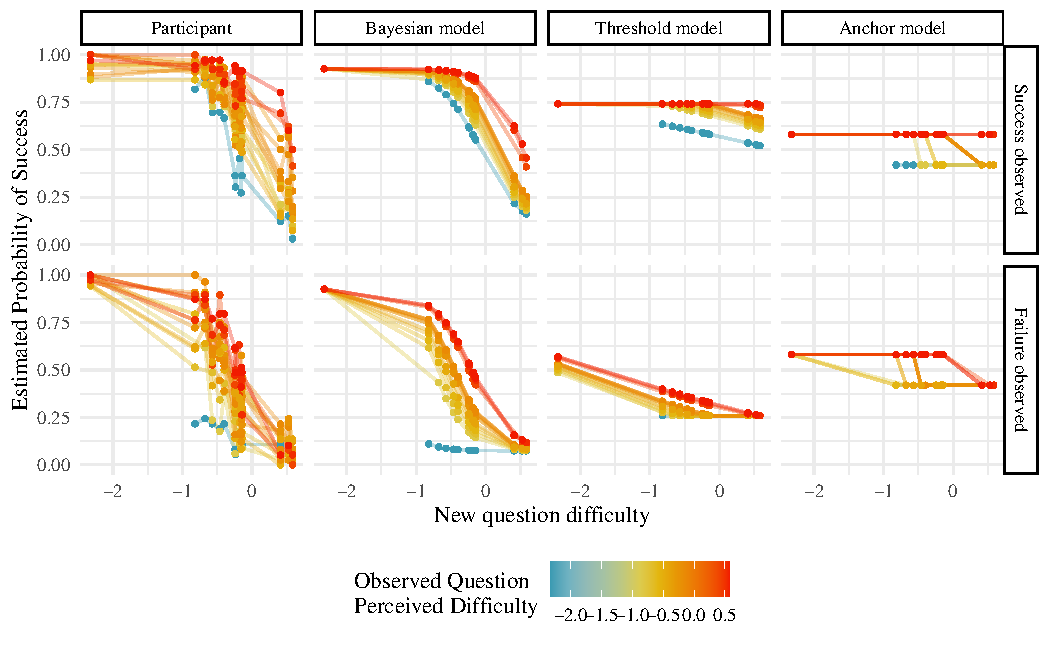
\includegraphics[width=0.9\linewidth]{../figures/S1-fig-model-comparison-1}

}

\caption{Model comparison. Each data point is a pair of two questions (one observed question and one evaluated question). The left column shows participants' average predictions, while the remaining columns show predictions from the Bayesian model, Threshold model, and Anchor model respectively. The top row shows trials where success was observed, and the bottom row shows trials where failure was observed. Lines connect predictions for the same observed question across different evaluated questions, colored by the observed question's perceived difficulty.}\label{fig:S1-fig-model-comparison}
\end{figure}

% To test \textbf{H4} and \textbf{H5}, we computed the Bayesian information criterion (BIC) using the maximum log-likelihood for each fitted model, which applies a penalty for model complexity. The Main Model, when fitted to the complete dataset, outperformed both alternative models (\(BIC_{Bayes}\) = 16,063.72; \(BIC_{Threshold}\) = 19,411.92; \(BIC_{Anchor}\) = 18,259.96), confirming \textbf{H4} and \textbf{H5} respectively. The difference between the BIC of the Main Model and that of the next best heuristic model (Anchor Model) was 2,196.24, which indicates very strong evidence in favor of our Main Model according to the standard interpretation criteria (Raftery, 1995).

% \subsection{Exploratory Analysis}\label{exploratory-analysis}

% As further exploratory analysis, we investigated several research questions. The first was whether if we divide the data by whether the participants observed a virtual agent's success or failure, participants' mean predictions of the probabilities of success still correlate with the true conditional probabilities (\textbf{RQ1}). In other words, we tested whether Hypothesis 2 was robust to the success/failure condition. We divided the data by whether success or failure was observed, and then for each data frame ran a linear model identical to the one used to test H2, with average estimated conditional probability as the dependent variable and true conditional probability as the independent variable. For both success and failure observations the regression estimate of true conditional probability was significantly positive and close to 1 (Success: \(\beta\) = 0.84, t(208) = 22.79, p \textless{} .001, Adjusted \(R^2\) = 0.71. Failure: \(\beta\) = 0.83, t(208) = 21.26, p \textless{} .001, Adjusted \(R^2\) = 0.68.)

% In another robustness test of our analyses for H2, we analyzed participants' binary answers at the trial level. We ran a logistic mixed-effects model with participants' predictions as the dependent variable and the true conditional probability as the independent variable. We included random intercepts for the observed question, the evaluated question, for the outcome observed (success/failure) and we also included random slope and intercept for participants. We found that, at each trial, participants' binary predictions of success were correlated with with the true probabilities of success (b= 1.65, z = 21.11, p \textless{} .001).

% We finally investigated how the models compared when we allowed to the parameters to differ for each individual rather than fixing them across all individuals. We did this because individuals may have different prior distributions of competence in the population. They may also have different priors about the role of luck in answering the questions. We therefore tested whether the main model fit individual level data better than heuristic model 1 (\textbf{RQ2}) and heuristic model 2 (\textbf{RQ3}). We used a maximum likelihood optimization to estimate the best free parameters for each participant. On average, our main model explained the behaviour of participants significantly better than Heuristic 1 (\(BIC_{Bayes}\) = 70.66 ± 20.38; \(BIC_{Threshold}\) = 87.97 ± 17.81; t(216) = -16.93, p \textless{} .001, paired t-test) and Heuristic 2 (\(BIC_{Anchor}\) = 80.86 ± 19.80; t(216) = -10.84, p \textless{} .001, paired t-test). The Bayesian model was the best model for 72\% of participants whereas the Heuristic 1 accounted for 6\% and the Heuristic 2 accounted for 21\%.

% \subsection{Exploring Response Time Data}\label{exploring-response-time-data}

% We began by testing, for any pair of participants who got the same question correct (for all questions), in what proportion of these pairs the one who answered faster achieved a higher total score. For each pair, we identified which participant responded faster and then compared their total scores across the task. Pairs with identical response times were excluded (only 0.072\% of the pairs). We then calculated the proportion of pairs in which (a) the faster participant achieved a higher total score, (b) both participants achieved the same total score, and (c) the faster participant achieved a lower total score. We found that in 52.5\% of the pairs, the participant who got the right answer faster had a higher total score, in 10.2\% of the pairs participants tied, and in 37.3\% of pairs the participant who reached the correct answer faster had a lower total score.

% In order to further investigate whether participants who were faster than their peers on a question they solved tended to be more accurate on other questions, we constructed a model which used participants' relative (scaled) speed on any particular question to predict accuracy on all other questions. We first defined an anchor question \emph{q} for each participant as any question they answered correctly. For each such \emph{q}, we computed that participant's relative speed on \emph{q} by z-scoring the negative response time within that question among the subset who were correct on \emph{q} (so higher values mean faster than peers who also solved \emph{q}). We then created, for every participant--anchor pair (id, \emph{q}), one row for each other target question \emph{r} \(\neq\) \emph{q}, with the binary outcome being whether the participant was correct on \emph{r}. From this dataset we fit a mixed-effects logistic regression predicting success on \emph{r} with a fixed effect for relative speed on \emph{q} and random effects for participant, \emph{r}, and \emph{q}.

% We found that the fixed effect for relative speed on anchor question \emph{q} was very small and not significant (\(\beta\) = 0.03, p = 0.193). Being faster than peers on a question a participant solved did not meaningfully predict accuracy on other questions.

% Finally, we fit another mixed-effects logistic regression to investigate whether response time on a question predicted accuracy on that question across participants and items. Here we found that response time had a significant negative effect on accuracy (\(\beta\) = -0.10, p \textless{} .001), indicating that longer response times were associated with lower accuracy. Converting from log-odds, each one-second increase in response time corresponded to a 9.88\% decrease in the odds of answering correctly.

\section{Study 2}\label{study-2}

Study~2 tests whether observers incorporate response time as an additional cue to numerical competence, beyond accuracy. Response time is theoretically ambiguous: faster correct answers may signal fluency, but longer times can also reflect greater caution or verification \citep{Hedge-2018,Goldhammer-2011,Richardson-2022,Berke-2023}. To isolate the diagnostic value of speed, we introduced two observation conditions: in the Fast condition the target had 20~s to respond, whereas in the Slow condition the target had 40~s. The key idea is that observing a correct answer should be slightly more diagnostic of competence when it occurs under a tighter time limit. However, observing a failure should be less diagnostic of incompetence in the Fast condition compared to the same question in the Slow condition. All else equal, being in the Fast condition should lead to higher estimation of competence.

We pre-registered the following hypotheses:

\textbf{H1.} Participants accurately assess the difficulty of correctly answering the observed questions.

\textbf{H2a.} For a given pair of Quiz 1 and Quiz 2 questions, among participants who correctly answered the Quiz 2 question, those who answered under a 20-second time limit have a higher chance of answering the Quiz 1 question than those who answered under a 40-second time limit.

\textbf{H2b.} For a given pair of Quiz 1 and Quiz 2 questions, among participants who failed the Quiz 2 question, those who failed under a 20-second time limit have a higher chance of answering the Quiz 1 question than those who failed under a 40-second time limit.

\textbf{H3.} On average, participants' predictions of the probabilities of success on different evaluated questions, given success or failure within the 20-second or 40-second time limit on an observed question, are significantly correlated with true conditional probabilities.

\textbf{H4a.} For a given pair of Quiz 1 and Quiz 2 questions, participants’ predictions of the probabilities of success on different evaluated questions will be higher for correctly answered observed questions under 20 seconds rather than under 40 seconds.

\textbf{H4b.} For a given pair of Quiz 1 and Quiz 2 questions, participants’ predictions of the probabilities of success on different evaluated questions will be higher for incorrectly answered observed questions under 20 seconds rather than under 40 seconds.


% In this second experiment, we investigated whether people use the time-taken to answer a question as a cue for competence. The previous experiment focused exclusively on accuracy as the signal of competence, only telling participants whether the evaluated individual got a particular question right or wrong. Everyday judgments of competence may also depend on effort: we intuitively believe that if two individuals both succeed at a task, the one who does so with less effort demonstrates greater competence. Yet, effort is not directly observable for many tasks, particularly cognitive tasks. One plausible proxy is time-taken – we may interpret shorter response times as evidence of greater fluency or ability, and there is evidence that speed is associated with competence in  arithmetic (Roy et al. 2025, Cheng et al., 2021, Prakash and Heckler, 2025). Conversely however, some studies suggest an opposite inference: people sometimes view slower, more deliberate responses as more competent because they may indicate more careful or complex reasoning (e.g. Richardson \& Keil, 2022;  Berke \& Jara-Ettinger, 2022). There are competing intuitions about how time-taken affects inferences about others’ competence.

% In the exploratory analysis of response times and accuracy on the arithmetic questions in Study 1, we did not find any strong evidence that faster responders were more competent, investigating this through various statistical tests. 

% We propose, in line with Hedge et al (2018), that this ambiguity arises because while more competent people are more efficient, they may also be more vigilant, taking more time to check their answers before submitted. This may be because they incur a greater reputational cost (decrease in perceived competence) from inaccurate answers. These counteracting negative and positive effects of competence and response time could explain the weak and inconsistent correlations between speed and competence in Study 1.

% The present experiment is designed to test whether people's inferences about competence from speed match the true relationship between competence and speed on an arithmetic test. We do this by creating two speed conditions – Fast (20 seconds) and Slow (40 seconds). Crucially, in the Fast condition, vigilance is very restricted, minimising the negative correlation between competence and speed, whereas in the Slow condition, competent people have more time for vigilance so the negative correlation remains. We predict that, for the same question, a correct answer within a 20 second time limit (Fast condition) indicates higher competence than answering it within a 40 second time limit (Slow condition), and that people will make this same inference. 

% [example to introduce the competing intuitions that taking long can imply deep thinking and vigilance or can imply incompetence, motivating our experimental setup: in an exam hall the people who hand in early - are they geniuses or did they not know enough to carry on]

% We pre-registered the following hypotheses:

% H1: Participants accurately assess the difficulty of correctly answering the observed questions.
% H2a: For a given pair of Quiz 1 and Quiz 2 questions, among participants who correctly answered the Quiz 2 question, those who answered under a 20-second time limit have a higher chance of answering the Quiz 1 question than those who answered under a 40-second time limit.
% H2b: For a given pair of Quiz 1 and Quiz 2 questions, among participants who failed the Quiz 2 question, those who failed under a 20-second time limit have a higher chance of answering the Quiz 1 question than those who failed under a 40-second time limit.
% H3: On average, participants' predictions of the probabilities of success on different evaluated questions, given success or failure within the 20 second or 40 second time limit on an observed question, are significantly correlated with true conditional probabilities.
% H4a: For a given pair of Quiz 1 and Quiz 2 questions, participants’ predictions of the probabilities of success on different evaluated questions will be higher for correctly answered observed questions in under 20 seconds rather than under 40 seconds.
% H4b: For a given pair of Quiz 1 and Quiz 2 questions, participants’ predictions of the probabilities of success on different evaluated questions will be higher for incorrectly answered observed questions in under 20 seconds rather than under 40 seconds.
% H1m: Even participants with minimal arithmetic ability can, for different observed questions, accurately assess the difficulty of these questions.
% H3m: Even for participants with minimal arithmetic ability, their average predictions of the probabilities of success on different evaluated questions, given success or failure within the 20 second or 40 second time limit on an observed question, are significantly correlated with true conditional probabilities.
% [For H1m and H3m ‘minimal arithmetic ability’ is defined as 30\% of participants with the lowest scores over the whole Quiz Phase (three quizzes)]
% H3i: At the trial level, participants' predictions of the probabilities of success on different evaluated questions, given success or failure within the 20 second or 40 second time limit on an observed question, are significantly correlated with true conditional probabilities.

\subsection{Methods}\label{methods-2}

\subsubsection{Participants}\label{participants-2}

We recruited 400 U.S. participants via Prolific Academic. As in Study~1, we excluded participants who passed the cheat-test item (N = 25) or reported using calculation aids (N = 18); no one failed the attention check (N = 0). We additionally implemented bot-detection measures (N = 7). The final sample comprised N = 354 (224 women; \(M_{Age}=41.7\), \(SD_{Age}=12.7\)).

\subsubsection{Behavioral task}\label{behavioral-task-2}

As in Study 1, all participants completed both phases of the experiment - the Quiz Phase and the Judgement Phase. In Study 2, however, the Quiz Phase was completed first such that participants experienced answering the questions within different time limits before making judgements. 
During the Quiz Phase, participants took three arithmetic quizzes, each consisting of 5 questions. First, each participant took Quiz 1, a slow quiz where they had 40 seconds to answer each question. Then each participant took Quiz 2 which could either be fast (20 seconds per question) or slow (40 seconds per question), with the time limit randomly assigned across participants. Finally,  each participant took Quiz 3 which was assigned whichever time limit they did not have for Quiz 2. There was a distinct set of questions for each of the three quizzes (but constant across participants) and within each quiz, questions were presented in randomised order. At no point were participants shown the correct answers.
In other words, we had two conditions randomised across participants: A “Fast Slow” Condition, where Quiz 1 allowed 40 seconds per question, Quiz 2 allowed 20 seconds per question (Fast) and Quiz 3 allowed 40 seconds per question (Slow), and a “Slow fast” Condition where Quiz 1 allowed 40 seconds per question, Quiz 2  allowed 40 seconds per question (Slow) and Quiz 3 allowed 20 seconds per question (Fast).

Quiz 1 and 2 performances were used as the ‘true performance data’, and compared to the judgements that people made in the Judgement Phase, where the same questions were used for the evaluated questions (Quiz 1) and the observed questions (Quiz 2). Quiz 3 was intended to ensure each participant experienced how difficult it is to answer questions within the different time limits. The cheat-test question was placed at the end of Quiz 1, but not included in any analysis not used as an evaluated question. As in Study 1, participants were instructed to only use mental calculation and told that their compensation did not depend on their performance.
The Judgement Phase was almost identical to that in Study 1, except now participants also observed different time limits in which the virtual agent succeeded or failed on a given question (e.g. Participant id58 had a 40 second time limit to answer the following question, and we recorded that they got it right: 2646 + 3271.). Below the observed question, participants were presented the 5 questions from Quiz 1 in random order and asked to tick whether or not the virtual agent would succeed within the given limit. The perceived difficulty prompt for the observed question also integrated the time limit (e.g. Out of 100 participants, how many do you think got the question 2646 + 3271 right within 40 seconds?). Participants assessed 5 virtual agents, with different observed question and time limit combinations for each, randomly assigned and balanced across participants.

\subsection{Results}\label{results-2}

We first tested if participants were able to assess the difficulty of correctly answering the observed questions. We collected judgement of difficulty on the quiz 2 questions only as quiz 1 were materials from the first study. The analysis is not subdivided by time condition: both in the judgement phase and in the questionnaire phase, participants were presented with each condition half the time. A linear mixed effect model with random slope and intercept for participants showed that participants' estimations correctly tracked the difficulty of answering each question (H1: \(\beta\) = 0.39, t(313.06) = 16.85, p \textless{} .001).

To determine if the time condition in Quiz 2 provided information about the probability of answering correctly a question of the Quiz 1, we created pairs of Quiz 1 and Quiz 2 questions (e.g Q1.1-Q2.1, Q1.1-Q.2.2, etc.) from participants' answers. Note that this mirror the structure of the judgement phase: while H2a and H2b test if the time condition provide information (for correct and incorrect questions respectively), H4a and H4b test if participants rely on the time condition when making a judgement. We ran two logits mixed-effect models: one among participants who answered a given Quiz 2 question correctly and one among those who answered it incorrectly. In both models, the dependent variable was a binary variable coding if the question from Q1 was correctly answered and the independent variable was a factor coding if the Q2 question was solved (H2a) or failed (H2b) under the Fast or the Slow condition. We controlled for the specific pair with a random effect (therefore comparing for the same pair, the effect of solving/failing under the fast condition compared to the slow), the model also include random intercepts for participants. H2a was restricted to trials where the Q2 question was solved and H2b was restricted to trials where the Q2 question was failed. We found that for a given pair of Quiz 1 and Quiz 2 questions, among participants who correctly answered the Quiz 2 question, those who answered under a 20-second time limit have a higher chance of answering the Quiz 1 question than those who answered under a 40-second time limit (H2a: b = 0.51, z = 2.15, p = 0.031). Among participants who failed the Quiz 2 question, those who failed under a 20-second time limit also had a higher chance of answering the Quiz 1 question compared to those who failed under a 40-second time limit (H2b: b = 0.71, z = 2.63, p = 0.009). This indicate that, no matters the outcome on the Quiz 2 question, participants should attribute higher chance of success to participants in the Fast condition, although the effect is relatively small.

We replicated the analysis of study 1 and found that, on average, participants' predictions of the probabilities of success on different evaluated questions, given success or failure within the 20 second or 40 second time limit on an observed question, are significantly correlated with true conditional probabilities (H3: \(\beta\) = 0.89, t(98) = 19.47, p \textless{} .001, Adjusted \(R^2\) = 0.79). As shown in Figure \ref{fig:S2-fig-behav}, participants' estimations closely tracked the true conditional probabilities across both time conditions.

\begin{figure}

{\centering 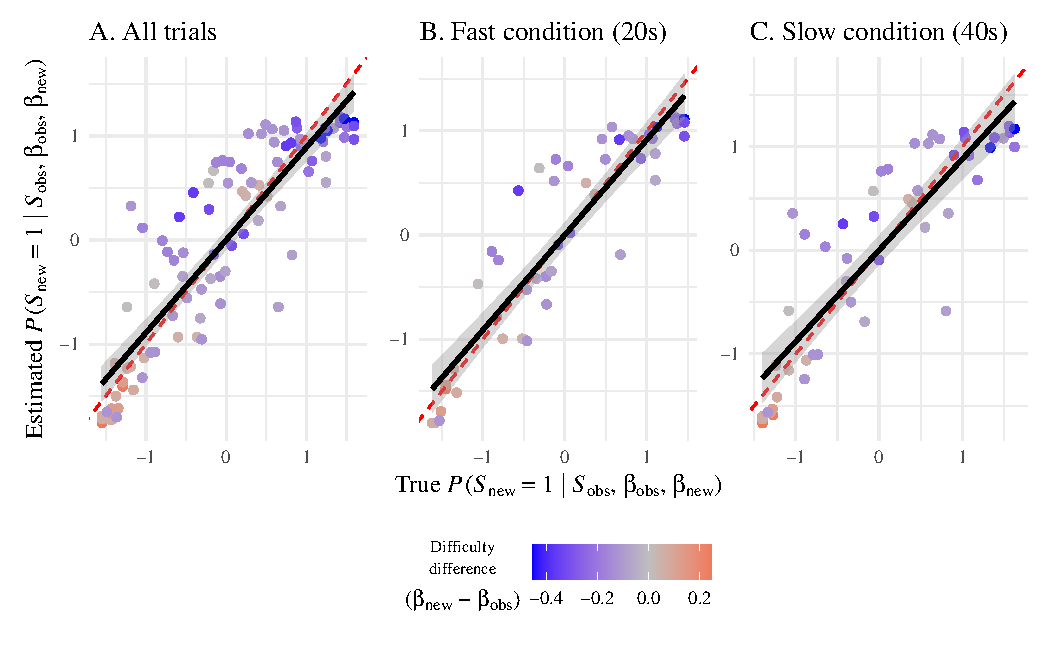
\includegraphics[width=0.9\linewidth]{../figures/S2-fig-behav-1}

}

\caption{Estimated Conditional Probability versus True Conditional Probability in Study 2. Each data point is a pair of two questions. The red line represents the optimal prediction while the dark line represents the fit of the linear models. Panel A shows all trials combined, panel B shows trials in the Fast condition (20-second time limit), and panel C shows trials in the Slow condition (40-second time limit). Points are colored by the difficulty difference between the evaluated and observed questions.}\label{fig:S2-fig-behav}
\end{figure}

Mirroring the analyses of H2a and H2b, we tested if participants took into account the information provided by the time condition when predicting success/failure on evaluated Quiz 1 questions. Similar models than H2a and H2b were estimated, but with participants' binary predictions as the dependent variable and the observed time condition as the independent variable (still controlling for the pair presented and restricting the analyses among success/failure observed). Results show that participants do not take into account the information provided by the time condition when observing a correct answer under 20 second compared to 40 second (H4a: b = 0.17, z = 1.53, p = 0.125) or when observing an incorrect answer (H4b: b = 0.15, z = 1.62, p = 0.104).

We further tested if our results for H1 and H3 were robust when testing predictions of participants with minimal arithmetic ability (defined as the bottom 30\% score in the questionnaire). Participants with minimal arithmetic ability can both accurately predict the difficulty of each question (H1m: \(\beta\) = 0.32, t(88.04) = 8.16, p \textless{} .001) and predict the conditional probabilities of success on evaluated questions (H3m: \(\beta\) = 0.88, t(98) = 18.73, p \textless{} .001, Adjusted \(R^2\) = 0.78).

Moreover, participants' predictions of the conditional probabilities of success were still correlated with the true probability when analyzed at the trial level (H3i: b = 1.95, z = 46.19, p \textless{} .001).

\section{General discussion and conclusion}\label{general-discussion-and-conclusion}

The capacity to infer the competence and knowledge of others is a core component of social cognition. Our main focus was to test whether inferences about competence are consistent with normative Bayesian reasoning but our paradigm also allows us to test whether participants make judgments that approximate objective conditional probabilities well. Study 1 replicate previous 

show that people can predict with a high degree of accuracy the conditional probability that a person knows the answer to a trivia question from a minimal amount of information---whether or not they know one other piece of information. This confirms that even a single observation can drive major updates in competence assessment, depending on the diagnosticity of the observed performance (e.g., success on a very difficult item). These studies also provide evidence that inferences of competence are well approximated by a Bayesian model which optimally integrates novel information with prior expectations. By contrast, plausible heuristics, corresponding to lesioned versions of the Bayesian model, do not account as well for most participants' behavior. These two findings---accurate judgments, and reliance on normative inferences---are relatively independent, as applying non-normative heuristics sometimes results in accurate judgments, while normative inferences can produce biased answers when the generative model or the parameters are not well calibrated.

Our research opens new directions in understanding the fundamental mechanisms of social cognition. Building on prior literature establishing the importance of past accuracy and difficulty cues, the present research offers a systematic, computational account of how people utilize this information. We show that in a naturalistic paradigm, reliable cues, even if they are minimal, allow participants to form very accurate estimations of competence, in line with Bayesian principles. Future research could address the question of how participants weigh and integrate multiple cues of competence of varying diagnosticity.

\printbibliography

\end{document}
